%%%%%%%%%%%%%%%%%%%%%%%%%%%%%%%%%%%%%%%%%%%%%%%%%%%%%%%%%%%%%%%%%%%%%%%%
%     LaTeX source code to approximate a Draft NIST Technical report
%	  Instructions for authors: tinyurl.com/techpubsnist 
%	DOI watermark will be added on final PDF
% 	Developed by K. Miller, kmm5@nist.gov 
%	Last updated: 22-March-2019
%%%%%%%%%%%%%%%%%%%%%%%%%%%%%%%%%%%%%%%%%%%%%%%%%%%%%%%%%%%%%%%%%%%

%%%%%%%%%%%%%%%%%%%%%%
% Template further altered by Armen Amirkhanian
% for use with UA lab courses in an effort to 
% have a standardized format for lab documents
% Last update 9-April-2020
%
% TODO:
% --Get the appendices to dynamically link, tocloft causes problems
%%%%%%%%%%%%%%%%%%%%%%

\documentclass[12pt]{article}
\usepackage{amsmath}
\usepackage{amsfonts}   % if you want the fonts
\usepackage{amssymb}    % if you want extra symbols
\usepackage{graphicx}   % need for figures
\usepackage{xcolor}
\usepackage{bm}
\usepackage{secdot}		
\usepackage{mathptmx}
\usepackage{float}
\usepackage[utf8]{inputenc}
\usepackage{textcomp}
\usepackage[hang,flushmargin,bottom]{footmisc} % footnote format
\usepackage{xspace}
%\usepackage{lineno}
\usepackage{ragged2e}
\usepackage{parskip}
\usepackage{textcomp}
\usepackage{environ}
\usepackage{multirow}
\usepackage{textgreek}

\usepackage{tikz}
\usetikzlibrary{shapes.geometric, arrows}
\tikzstyle{startstop} = [rectangle, rounded corners, minimum width=2cm, minimum height=1cm,text centered, draw=black, fill=red!20]
\tikzstyle{arrow} = [thick,->,>=stealth]

\usepackage{titlesec}
\titleformat{\section}{\normalsize\bfseries}{\thesection.}{1em}{}	% required for heading numbering style
\titleformat*{\subsection}{\normalsize\bfseries}

\usepackage{tocloft}	% change typeset, titles, and format list of appendices/figures/tables
\renewcommand{\cftdot}{}	
\renewcommand{\contentsname}{Table of Contents}
\renewcommand{\cftpartleader}{\cftdotfill{\cftdotsep}} % for parts
\renewcommand{\cftsecleader}{\cftdotfill{\cftdotsep}}
\renewcommand\cftbeforesecskip{\setlength{4pt}{}}
\addtolength{\cftfignumwidth}{1em}
\renewcommand{\cftfigpresnum}{\figurename\ }
\addtolength{\cfttabnumwidth}{1em}
\renewcommand{\cfttabpresnum}{\tablename\ }
\setlength{\cfttabindent}{0in}    %% adjust as you like
\setlength{\cftfigindent}{0in} 

\usepackage{enumitem}         % to control spacing between bullets/numbered lists

\usepackage[numbers,sort&compress]{natbib} % format bibliography 
\renewcommand{\bibsection}{}
\setlength{\bibsep}{0.0pt}

\usepackage[hidelinks]{hyperref}
\hypersetup{
	colorlinks = true,
urlcolor ={blue},
citecolor = {.},
linkcolor = {.},
anchorcolor = {.},
filecolor = {.},
menucolor = {.},
runcolor = {.}
pdftitle={},
pdfsubject={},
pdfauthor={},
pdfkeywords={}
}
\urlstyle{same}

\NewEnviron{letter}{%
\begin{quote}
\fbox{%
\begin{minipage}{\linewidth}
\setlength{\parskip}{\baselineskip}
%\letterfont
\BODY
\end{minipage}
}
\end{quote}
}

\usepackage{epstopdf} % converting EPS figure files to PDF

\usepackage{fancyhdr, lastpage}	% formatting document, calculating number of pages, formatting headers
\setlength{\topmargin}{-0.5in}
\setlength{\headheight}{39pt}
\setlength{\oddsidemargin}{0.25in}
\setlength{\evensidemargin}{0.25in}
\setlength{\textwidth}{6.0in}
\setlength{\textheight}{8.5in}

\usepackage{caption} % required for Figure labels
\captionsetup{font=small,labelfont=bf,figurename=Fig.,labelsep=period,justification=raggedright} 

%%%%%%%%%%% !!!!!REQUIRED - FILL OUT METADATA HERE !!!!!!!! %%%%%%%%%%%%%%
%%%%%%%%%%%%%%%%%%%%%%%%%%%%%%%%%%%%%%%%%%%%%%%%%%%%%%%%%%%%%%%%%%%%%%%%%%
\newcommand{\CourseNum}{CE262}
\newcommand{\CourseName}{Civil Engineering Materials}
\newcommand{\LabTitle}{Concrete Mixing and Testing}
\newcommand{\LastUpdate}{Fall 2020}

%%%%%%%%%%%%%%%%%%%%%%%%%%%%%%%%%%%%%%%%%%%%%%%%%%%%%%%%%%%%%%%%%%%%
%   	BEGIN DOCUMENT 
%%%%%%%%%%%%%%%%%%%%%%%%%%%%%%%%%%%%%%%%%%%%%%%%%%%%%%%%%%%%%%%%%%%%
\begin{document}
	\urlstyle{rm} % Format style of \url   
%\linenumbers
\begin{titlepage}
\begin{flushright}
\LARGE{\textbf{\CourseNum{} -- \CourseName}}\\
\vfill
\Huge{\textbf{\LabTitle}}\\
    \vfill
%%%%%%%%%%%%%%%%%%%%%%%%%%%%%%%%%%%%%%%%%%%%%%%%%%%%%%%%%%%%%%%%%%%%
%	Authors - add complete list of authors, affiliations will be 
%   added on title page
%%%%%%%%%%%%%%%%%%%%%%%%%%%%%%%%%%%%%%%%%%%%%%%%%%%%%%%%%%%%%%%%%%%%
    \large Dr. Armen Amirkhanian, P.E.\\
\vfill
%%%%%%%%%%%%%%%%%%%%%%%%%%%%%%%%%%%%%%%%%%%%%%%%%%%%%%%%%%%%%%%%%%%%
%	The DOI is automated based on metadata.	
%%%%%%%%%%%%%%%%%%%%%%%%%%%%%%%%%%%%%%%%%%%%%%%%%%%%%%%%%%%%%%%%%%%%
\normalsize This work is licensed under the Creative Commons Attribution-ShareAlike 4.0 International License. To view a copy of this license, visit:
\href{http://creativecommons.org/licenses/by-sa/4.0/}{http://creativecommons.org/licenses/by-sa/4.0/}.

\includegraphics[width=0.07\textwidth]{cc.eps}
\includegraphics[width=0.07\textwidth]{by.eps}
\includegraphics[width=0.07\textwidth]{sa.eps}
\vfill

\includegraphics[width=0.3\linewidth]{Logo.eps}\\ 
 
  
\end{flushright}
\end{titlepage}

\begin{titlepage}
\begin{center}
\normalsize 
Certain commercial entities, equipment, or materials may be identified in this document in order to describe an experimental procedure or concept adequately. Such identification is not intended to imply recommendation or endorsement by The University of Alabama or the listed authors, nor is it intended to imply that the entities, materials, or equipment are necessarily the best available for the purpose.\\
\vfill
Any opinions or recommendations are solely those of the author(s) and do not represent the official view or policy of The University of Alabama.
\end{center}
\begin{flushright}
\vfill
\normalsize 
This document was last updated in \textbf{\LastUpdate} and should contain \textbf{\pageref{LastPage}} pages of content exclusive of these title pages, abstract, and other front matter. If the document appears to be incomplete, please contact the author(s).\\
\vfill
Science is very important to me, but I also like to stress that you have to be well-rounded. One's love for science doesn't get rid of all the other areas. I truly feel someone interested in science is interested in understanding what's going on in the world. That means you have to find out about social science, art, and politics.\\
\textit{Mae Jemison}
\end{flushright}
\end{titlepage}
%%%%%%%%%%%%%%%%%%%%%%%%%%%%%%%%%%%%%%%%%%%%%%%%%%%%%%%%%%%%%%%%%%%%
%   Start front matter - page number starts with "i"
%%%%%%%%%%%%%%%%%%%%%%%%%%%%%%%%%%%%%%%%%%%%%%%%%%%%%%%%%%%%%%%%%%%%
\pagenumbering{roman}
\section*{Abstract}
\normalsize Concrete is the most used man-made material in the world. It is figuratively and literally the foundation of civil engineering. For all of its applications, there is one common theme with any concrete mixture: water, cement, aggregates. Even minor changes in the ratios of these three materials can significantly affect the strength, durability, and performance of the resulting mixture.

\vfill
\section*{Keywords}
\normalsize concrete; mixture design; slump; unit weight; air content.\\
\pagebreak
%%%%%%%%%%%%%%%%%%%%%%%%%%%%%%%%%%%%%%%%%%%%%%%%%%%%%%%%%%%%%%%%%%%%
%   Table of Contents is required
% 	List of Tables & Figures required if more than 5 tables/figures
%%%%%%%%%%%%%%%%%%%%%%%%%%%%%%%%%%%%%%%%%%%%%%%%%%%%%%%%%%%%%%%%%%%%
\begin{center}
\tableofcontents
\pagebreak
\listoftables
\listoffigures
\end{center}
\pagebreak
\section*{Required Specifications}
The following specifications are required to complete this laboratory exercise:
\begin{description}
\item[ACI 211.1] Standard Practice for Selecting Proportions for Normal, Heavyweight, and Mass Concrete
\item[ASTM C138] Standard Test Method for Density (Unit Weight), Yield, and Air Content (Gravimetric) of Concrete
\end{description}

The following specifications are optional, but they are listed here in the event more information is needed to complete the laboratory exercise:
\begin{description}
\item[ASTM C125] Terminology Relating to Concrete and Concrete Aggregates
\item[ASTM C127] Standard Test Method for Relative Density (Specific Gravity) and Absorption of Coarse Aggregate
\item[ASTM C128] Standard Test Method for Relative Density (Specific Gravity) and Absorption of Fine Aggregate
\end{description}
\pagebreak
%%%%%%%%%%%%%%%%%%%%%%%%%%%%%%%%%%%%%%%%%%%%%%%%%%%%%%%%%%%%%%%%%%%%
%   Start body of text - page number starts with "1"
%%%%%%%%%%%%%%%%%%%%%%%%%%%%%%%%%%%%%%%%%%%%%%%%%%%%%%%%%%%%%%%%%%%%
\section{Concrete Mixture Design}
\label{sec:intro}
\pagenumbering{arabic}
\normalsize 
This laboratory exercise, compared perhaps to any other exercise you will ever do, is wide-open. You can do what you want! As you have seen, the process of calculating a concrete mixture design uses a significant amount of designer inputs so there are essentially an infinite number of valid mixture designs. In this exercise, you will design your own mixture using very broad requirements. It is very likely you will get a mixture that is ``bad'' (i.e. low slump, high slump, soup, etc) and that is okay. Your grade is not impacted by the quality of your concrete, just your process.

\subsection{Objectives}
\label{ssec:headingscap}
At the completion of this lab exercise section, you will have satisfied the following objectives:
\begin{enumerate}
    \item Design a concrete mixture following principles outlined in ACI 211.1
    \item Perform concrete mixture procedures and produce a concrete mixture based on design calculations
    \item Perform testing on a concrete mixture to characterize yield
    \item Perform calculations necessary to determine corrections needed to improve the concrete mixture design
\end{enumerate}

\subsection{Learning Outcomes}
At the completion of this lab exercise, you should be able to:
\begin{itemize}
    \item understand the concrete mixture design process as outlined in ACI 211.1
    \item understand the qualitative relationship of the concrete mixture constituents on mixture properties
    \item understand how to correct a concrete mixture design based on trial mixtures
    \item present calculated values in a useful and professional manner
\end{itemize}

\pagebreak
\subsection{Procedure}
The general process for batching and mixing concrete is straightforward. However, for this exercise, there will be a few specific criteria you will need to consider as you go through the process.

\subsubsection{Prior To Lab}
Before arriving to lab to complete the exercise, you should already have calculated the mixture you are going to produce. As you design your concrete mixture, you will need to account for the following restrictions:
\begin{itemize}
    \item Portland cement amount shall not exceed 800 lbs/yd$^3$
    \item w/c shall not be less than 0.31 nor greater than 0.90
    \item Assumed air content shall not exceed 4\%
\end{itemize}

While you have already characterized the coarse and fine aggregate sources in a previous laboratory exercise, you will use provided material properties (Appendix A) to perform the calculations. Both of the aggregate sources can safely be considered oven-dry. It is extremely important that you do not forget to account for the water absorption of the aggregate. This means that your \textbf{selected} water content will always be less than the \textbf{needed} water content. Refer to the course notes on how to account for this in your design process.

You may already realize that batching out an entire cubic yard of concrete is absurd and you are correct. For the lab trial, you will need to scale your batch size down to something manageable. We will go with a batch volume of 0.30 ft$^3$ instead of 27 ft$^3$. We scale the weights of each component down to the smaller size (Table \ref{tab:SSDexam}).

\begin{table}[h]
\begin{center}
\caption{Example concrete mixture design and associated lab-scale weights for mixing. All values in SSD conditions.}
\label{tab:SSDexam}
\begin{tabular}{rcc}
\hline
Constituent     & \multicolumn{1}{l}{Amount, lbs/yd$^3$} & \multicolumn{1}{l}{Amount, lbs} \\ \hline
Water           & 500                                    & 5.56                            \\
Portland Cement & 1000                                   & 11.11                           \\
Coarse Agg.     & 1500                                   & 16.67                           \\
Fine Agg.       & 800                                    & 8.89                            \\
Air             & \multicolumn{2}{c}{4\%}                                                  \\ \hline
\end{tabular}
\end{center}
\end{table}

As just mentioned, we need to account for the fact that our aggregates will absorb some of that 5.56 lbs of water we are adding. This is a problem because it can significantly affect the w/c of the mixture. For sake of the example, let's say the coarse aggregate has an absorption capacity of 4\% and the fine aggregate has an absorption capacity of 5\%. We would account for this as additional water needed for our mixture (Table \ref{tab:ODexam}). So, instead of adding 5.56 lbs of water as originally planned, we need to add a total of 6.67 lbs of water! We also will add slightly less aggregate. Forgetting to account for the absorption of the aggregates is the biggest mistake students make with this laboratory exercise.

\begin{table}[h]
\begin{center}
\caption{Example concrete mixture design and associated lab-scale weights for mixing. All values in OD conditions.}
\label{tab:ODexam}
\begin{tabular}{rcc}
\hline
Constituent     & \multicolumn{1}{l}{Amount, lbs/yd$^3$} & \multicolumn{1}{l}{Amount, lbs} \\ \hline
Water           & 500                                    & 5.56                            \\
Addl. Water     & 100                                    & 1.11 \\
Portland Cement & 1000                                   & 11.11                           \\
Coarse Agg.     & 1440                                   & 16.00                           \\
Fine Agg.       & 760                                    & 8.44                            \\
Air             & \multicolumn{2}{c}{4\%}                                                  \\ \hline
\end{tabular}
\end{center}
\end{table}

\subsubsection{Execution}
Once you arrive to the lab, you can begin to weigh out your four materials (i.e. water, cement, coarse and fine aggregate). You should weigh out the aggregates first and immediately add them to the mixer. Then, weigh out the water and portland cement in two separate buckets. Before starting the mixer, add about half\footnote{Straight up eyeball this. It does not have to be remotely close to half of the water, you just want the aggregates kind of wet. If you accidentally add all the water it is not the end of the world.} of your water to the aggregates in the mixer. This will help pre-wet the aggregates and coat the inside of the mixer with a film of water.

Keeping your hands, long hair, and/or loose clothing away from the drum of the mixer, start the machine and let the wet aggregate mix for approximately 21 seconds. Stop the mixer and add all of your portland cement. Start the mixer back up and as the drum is spinning slowly dump in the remaining water. The goal is to ``rinse'' the sides of the mixer as you dump in the water just to make sure as much cement as possible makes it into the mix.

How long does this mix for? Oh boy, this is where everyone and their brother has an opinion. Depending on the agency, client, specification, time of day, astrological sign, etc you'll get different answers. Here is a general recommendation:
\begin{itemize}
    \item Mix for about 2--3 minutes
    \item Turn off mixer and let the contents ``rest'' for about 1 minute
    \item Mix for an additional 2--3 minutes or until it looks like nothing is changing
\end{itemize}

\subsubsection{Yield}
This is one of the more difficult aspects of the mixture design process. You will take your just mixed concrete and see if the unit weight of the actual mixture matches the theoretical unit weight of your design. First, we need the total weight of all materials in our mixture design (refer back to Table \ref{tab:SSDexam}). We are adding four physical things, that have weight, to our mixture: water, portland cement, coarse and fine aggregate. If we sum up those weights, we get 3,800 lbs.

Next, we need to determine the actual unit weight of the concrete mixture. You will follow the general steps outlined in ASTM C138. We need a container of known volume and will use a metal bucket that has a volume of 0.25 ft$^3$. You will weigh the bucket empty, fill it up with concrete, and then weigh it full. The difference in weight is the unit weight of the concrete per 0.25 ft$^3$ which is readily converted to a unit weight in lbs/ft$^3$.

For sake of the example, let's say we measured our real-life concrete to have a unit weight of 135.9 lbs/ft$^3$. Using Eq. 3 in ASTM C138, we calculate a yield of 1.04 yd$^3$. This means we actually produced more concrete, by volume, than we had planned. Had our yield been exactly 1.00 yd$^3$, that would mean our theoretical values match the real-life. A common reason for this discrepancy is predicting the wrong air content. We had assumed 4\% air content. However, if we are getting more concrete, by volume, than we expected that likely means we have a higher air content!

If we calculate the air content using Eq. 7 of ASTM C138, we see that in our example, we actually ended up with 7.3\% air! Using this equation is a little bit tricky. You need the theoretical unit weight, $T$, which is the total mass of the designed mixture, 3,800 lbs, divided by the volume. A common mistake is to use a volume of 27 ft$^3$ but the volume, $V$, that is needed in the standard is only the volume of the physical constituents (i.e. everything except air). So the theoretical unit weight for this example is calculated using a total volume of 25.92 ft$^3$ which gives us a final value of 146.6 lbs/ft$^3$.

\subsubsection{Specimens}
You will cast a single specimen for testing in a later laboratory exercise. In the concrete industry, we often cast cylindrical specimens as the various tests we run are more consistently run with a cylindrical shape\footnote{Due to stress concentrations for sharp corners in shapes like cubes and rectangles.}. There are two common sizes of cylinders we use: 4 inch diameter and 8 inch height, and 6 inch diameter and 12 inch height. It is no coincidence that the diameter is exactly half of the height and the reason for this is based on stress distribution during testing\footnote{You can use the stuff you learn in AEM250 to actually derive why this is true!}. People in the industry refer to these two sizes as ``4 by 8'' and ``6 by 12'' cylinders.

You will, to the best of your ability, cast a single 4 by 8 cylinder with your concrete mixture. I say to the best of your ability because your mixture may be extremely difficult to work with! Just do the best you can to consolidate the concrete into the cylinder and strike-off the top so that it is smooth. Be sure to label the cylinder with your provided student information so that it can be identified in the later laboratory exercise.



\subsection{Summary}
You have successfully\footnote{Hey, it doesn't matter if you ended up with clumps, soup, or something in-between. You designed it from scratch and that is no easy feat!} designed and batched a concrete mixture. It is easy to make seemingly little mistakes in your calculations that can have a big impact on the final product. Regardless of the quality of your mixture, you hopefully have some better insight into the concrete mixture design process. 


\pagebreak
\section{Deliverables}
For this laboratory exercise, you will need to submit a single mixture design form following the general format of the example worksheets in Appendix B. Some of the details listed in the example, such as ``Class of concrete'' are not necessary for you to include. Your submission should be a single page
\begin{itemize}
    \item All specific gravities/relative densities used in the calculations
    \item Weights for 1 yd$^3$
    \item Weights for laboratory batch size (0.3 ft$^3$)
    \item NMAS of coarse aggregate
    \item Assumed slump and w/c
    \item Theoretical and measured unit weight
    \item Yield
\end{itemize}

A large part of this exercise is professional formatting. You will likely spend more time making the page(s) look good than performing the actual calculations and this is okay! Professional engineers will typically use software specifically designed to make nice sheets. However, there are still some firms and engineers that do it manually. Most of the time the entire page is created in MS Excel due to the insane number of rows and columns needed. Here are some DOs and DON'Ts to help guide you in making a professional submission:

\begin{itemize}
    \item DO be consistent with decimal places and where applicable, follow the ASTM/ACI rules for number of decimal places
    \item DO indicate units properly
    \item DON'T include extraneous fields that have values of ``N/a'' or similar
    \item DON'T use a font size smaller than 10pt
    \item DON'T use shading (i.e. shading alternating rows)
    \item DON'T use a cover page
\end{itemize}

%\section*{References}
%\addcontentsline{toc}{section}{References}
%\bibliographystyle{techpubs}
%\bibliography{References}

%%%%%%%%%%%%%%%%%%%%%%%%%%%%%%%%%%%%%%%%%%%%%%%%%%%%%%%%%%%%%%%%%%%%
%   Please use the techpubs BibTeX style when compiling bibliography, or follow the instructions on tinyurl.com/techpubsnist to format your .bib / .bbl file appropriately.
%%%%%%%%%%%%%%%%%%%%%%%%%%%%%%%%%%%%%%%%%%%%%%%%%%%%%%%%%%%%%%%%%%%%
\pagebreak

\section*{Appendix A1: Coarse Aggregate Datasheet}
\label{AppendixB}
\addcontentsline{toc}{section}{Appendix A1: Coarse Aggregate Datasheet}
\begin{center}
    \includegraphics[width=1\linewidth]{Coarse.eps}
\end{center}

\pagebreak

\section*{Appendix A2: Fine Aggregate Datasheet}
\label{AppendixB}
\addcontentsline{toc}{section}{Appendix A2: Fine Aggregate Datasheet}
\begin{center}
    \includegraphics[width=1\linewidth]{Fine.eps}
\end{center}

\pagebreak

\section*{Appendix B: Example Concrete Mixture Form}
\label{AppendixB}
\addcontentsline{toc}{section}{Appendix B: Example Concrete Mixture Form}
\begin{center}
    \includegraphics[width=1\linewidth]{1608_v11_1.eps}
\end{center}


%\pagebreak
%\section*{Appendix B: Change Log}
%\addcontentsline{toc}{section}{Appendix B: Change Log}
%This document was originally created on April 9, 2020. Any changes will be documented in this appendix.

\end{document}
%%%%%%%%%%%%%%%%%%%%%%%%%%%%%%%%%%%%%%%%%%%%%%%%%%%%%%%%%%%%%%%%%%%%
%   When referring to references in the text parenthetically, 
%	use the form “[1].” For example, “As Jones and Smith have shown [1];”
%	 however, when a reference is referred to non-parenthetically, use the form 
%	“. . . Ref. [1] . . .” (except at the beginning of a sentence where
%	“Reference [1] . . .” is the correct form).
%%%%%%%%%%%%%%%%%%%%%%%%%%%%%%%%%%%%%%%%%%%%%%%%%%%%%%%%%%%%%%%%%%%%

%%%%%%%%%%%%%%%%%%%%%%%%%%%%%%%%%%%%%%%%%%%%%%%%%%%%%%%%%%%%%%%%%%%%
%   Section references are “Sec. X”.
% 	“Section X” is used at beginning of sentence. 
%%%%%%%%%%%%%%%%%%%%%%%%%%%%%%%%%%%%%%%%%%%%%%%%%%%%%%%%%%%%%%%%%%%%

%%%%%%%%%%%%%%%%%%%%%%%%%%%%%%%%%%%%%%%%%%%%%%%%%%%%%%%%%%%%%%%%%%%%
%   Equation references are “Eq. (X)”.
% 	“Equation (1) is used at beginning of sentence.
%	Equations are numbered (#) on the right, per the standard LaTeX format
%%%%%%%%%%%%%%%%%%%%%%%%%%%%%%%%%%%%%%%%%%%%%%%%%%%%%%%%%%%%%%%%%%%%

%%%%%%%%%%%%%%%%%%%%%%%%%%%%%%%%%%%%%%%%%%%%%%%%%%%%%%%%%%%%%%%%%%%%
%   Tables should appear after they are mentioned in the text. 
%	Superscripted letters (a, b, c, etc.) should be used for table footnotes.
%%%%%%%%%%%%%%%%%%%%%%%%%%%%%%%%%%%%%%%%%%%%%%%%%%%%%%%%%%%%%%%%%%%%

%%%%%%%%%%%%%%%%%%%%%%%%%%%%%%%%%%%%%%%%%%%%%%%%%%%%%%%%%%%%%%%%%%%%
%   Figure references are “Fig. X”.
% 	“Figure X” is used at beginning of sentence. 
% 	Figures should appear after they are mentioned in the text.
%	Figures must have embedded alternate text or “alt text” in order 
%	to comply with Section 508 accessibility standards. 
%%%%%%%%%%%%%%%%%%%%%%%%%%%%%%%%%%%%%%%%%%%%%%%%%%%%%%%%%%%%%%%%%%%%